\subsection{Synthesis of the cyclopentanol conjugates\label{sec:HOcy5}}

\subsubsection{Synthesis of the 2-aminocyclopentan-1-ol head groups \compound{cmpd:HOcy5NH2_SS} and \compound{cmpd:HOcy5NH2_RR} \label{sec:HOcy5NH2}}

Synthesis of the cyclopentanol derivatives began with the synthesis of (1\textit{S},2\textit{S})-2-aminocyclopentan-1-ol \compound{cmpd:HOcy5NH2_SS} and (1\textit{R},2\textit{R})-2-aminocyclopentan-1-ol \compound{cmpd:HOcy5NH2_RR} (see \ref{sch:HOcy5NH2_synth}), using a procedure reported by Overman and Sugai\cite{Aube1992,Overman1985,Overman1985a}.
These precursors were synthesised by opening cyclopentene oxide \compound{cmpd:Ocy5} using (\textit{S})-1-phenylethan-1-amine \compound{cmpd:NH2MeBn} to give approximately equal amounts of two diastereomers, \compound{cmpd:HOcy5NHMeBn_SSS} and \compound{cmpd:HOcy5NHMeBn_RRS}, which were separated using column chromatography. 
The removal of the methylbenzyl groups proved more difficult than expected, with the conditions reported by Overman and Sugai\cite{Overman1985} yielding only a salt of the starting material.
After several attempts under various conditions (including using the free amine vs. the salt, varying the temperature, ensuring the dryness of the reagents and adding acetic acid), an approach using \ce{H2} gas was attempted (see \ref{tbl:HOcy5NH2_opt}). This proceeded smoothly at 5 atm to give the two enantiomers of 2-aminocyclopentan-1-ol, \compound{cmpd:HOcy5NH2_SS} and \compound{cmpd:HOcy5NH2_RR}, both in quantitative yield.

\begin{scheme}[H]
	\begin{center}
		\schemeref[Ocy5]{cmpd:Ocy5}
		\schemeref[NH2MeBn]{cmpd:NH2MeBn}
		\schemeref[HOcy5NHMeBn_RRS]{cmpd:HOcy5NHMeBn_RRS}
		\schemeref[HOcy5NHMeBn_SSS]{cmpd:HOcy5NHMeBn_SSS}
		\schemeref[HOcy5NH2_RR]{cmpd:HOcy5NH2_RR}
		\schemeref[HOcy5NH2_SS]{cmpd:HOcy5NH2_SS}
		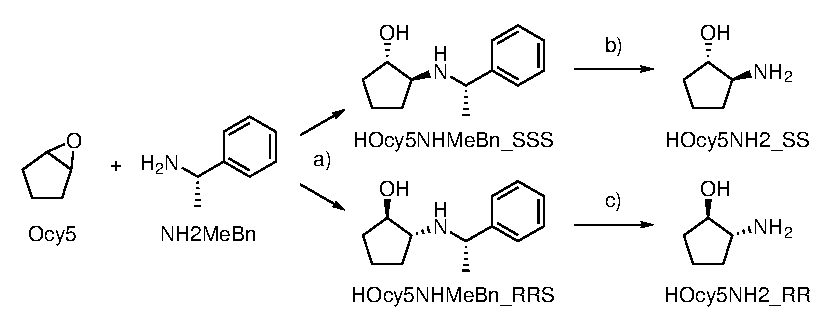
\includegraphics[scale=1]{HOcy5NH2_synth}
		\caption{Synthesis of (1\textit{S},2\textit{S})-2-aminocyclopentan-1-ol \compound{cmpd:HOcy5NH2_SS} and (1\textit{R},2\textit{R})-2-aminocyclopentan-1-ol \compound{cmpd:HOcy5NH2_RR}.
		a) \ce{AlMe3}, \ce{CH2Cl2}, 0 $^\circ$C,  
		\compound{cmpd:HOcy5NHMeBn_SSS} (\textit{SSS}): 35\%,
		\compound{cmpd:HOcy5NHMeBn_RRS} (\textit{RRS}): 32\%.
		b) See \ref{tbl:HOcy5NH2_opt}.
		c) \ce{Pd(OH)2}, MeOH, \ce{H2}, 5 atm, r.t., 1 d, >99\%.
		\label{sch:HOcy5NH2_synth}}
	\end{center}
\end{scheme}


\renewcommand{\arraystretch}{1.2}
\begin{table}[H]
  \centering
\begin{tabular}{|p{6cm}|p{2.4cm}|l|p{6cm}|}
\hline 
Conditions & Temperature and pressure & Time & Result \\ 
\hline 
\ce{\compound{cmpd:HOcy5NHMeBn_SSS}.HCl}, ammonium formate, 10\% Pd/C, DMF & r.t., 1 atm & 2 d & \compound{cmpd:HOcy5NHMeBn_SSS} salt \\ %LMO-2-047
\hline 
\compound{cmpd:HOcy5NHMeBn_SSS}, ammonium formate, 10\% Pd/C, DMF & r.t., 1 atm & 2 d & \compound{cmpd:HOcy5NHMeBn_SSS} salt \\ %LMO-2-048
\hline 
\ce{\compound{cmpd:HOcy5NHMeBn_SSS}.HCl}, ammonium formate, 10\% Pd/C, dry DMF & r.t., 1 atm & 2 d & \compound{cmpd:HOcy5NHMeBn_SSS} salt \\ %LMO-2-049
\hline 
\compound{cmpd:HOcy5NHMeBn_RRS}, ammonium formate, 10\% Pd/C, dry DMF & r.t., 1 atm & 2 d & \compound{cmpd:HOcy5NHMeBn_RRS} salt \\ %LMO-2-050
\hline 
\compound{cmpd:HOcy5NHMeBn_SSS}, ammonium formate, 10\% Pd/C, dry DMF & 70 $^{\circ}$C, 1 atm & 1 d & \compound{cmpd:HOcy5NHMeBn_SSS} salt \\ %LMO-2-051
\hline 
\compound{cmpd:HOcy5NHMeBn_SSS}, ammonium formate, 10\% Pd/C, dry DMF, AcOH & 70 $^{\circ}$C, 1 atm & 1 d & Complex mixture \\ %LMO-2-051
\hline 
\ce{\compound{cmpd:HOcy5NHMeBn_SSS}.HCl}, dry ammonium formate, 10\% Pd/C, dry DMF & 120 $^{\circ}$C, 1 atm & 7 d & Complex mixture \\ %LMO-2-054
\hline 
\ce{\compound{cmpd:HOcy5NHMeBn_SSS}.HCl}, \ce{Pd(OH)2}, MeOH, \ce{H2} & r.t., 1 atm & 1 d & \compound{cmpd:HOcy5NHMeBn_SSS} salt \\ %LMO-2-056
\hline 
\ce{\compound{cmpd:HOcy5NHMeBn_SSS}.HCl}, \ce{Pd(OH)2}, MeOH, \ce{H2} & r.t., 3.4 atm & 1 d & \compound{cmpd:HOcy5NH2_SS} salt, \compound{cmpd:HOcy5NHMeBn_SSS} salt, and an unidentified compound (approx. 7:2:10 by $^1$H NMR) \\ %LMO-2-055
\hline 
\compound{cmpd:HOcy5NHMeBn_SSS}, \ce{Pd(OH)2}, MeOH, \ce{H2} & r.t., 5 atm & 1 d & \compound{cmpd:HOcy5NH2_SS}, >99\% yield \\ %LMO-2-057
\hline 
\end{tabular} 
\caption{Conditions attempted for the synthesis of (1\textit{S},2\textit{S})-2-aminocyclopentan-1-ol \compound{cmpd:HOcy5NH2_SS} and (1\textit{R},2\textit{R})-2-aminocyclopentan-1-ol \compound{cmpd:HOcy5NH2_RR} (see \ref{sch:HOcy5NH2_synth}).\label{tbl:HOcy5NH2_opt}} 
\end{table}

\subsubsection{Initial branching route\label{sec:init_branch}}

An initial retrosynthesis of the conjugates is shown in \ref{sch:HOcy5NH4_retro_A}, and follows a similar path to previous conjugates.

\begin{scheme}[H]
	\begin{center}
		\schemeref[HOcy5NH2_RR]{cmpd:HOcy5NH2_RR}
		\schemeref[HOcy5NH4Br_RR]{cmpd:HOcy5NH4Br_RR}
		\schemeref[HOcy5NH4N3_RR]{cmpd:HOcy5NH4N3_RR}
		\schemeref[HOcy5NH4CipMe_RR]{cmpd:HOcy5NH4CipMe_RR}
		\schemeref[HOcy5NH4T4Cip_RR]{cmpd:HOcy5NH4T4Cip_RR}
		\schemeref[HOcy5NH2_SS]{cmpd:HOcy5NH2_SS}
		\schemeref[HOcy5NH4Br_SS]{cmpd:HOcy5NH4Br_SS}
		\schemeref[HOcy5NH4N3_SS]{cmpd:HOcy5NH4N3_SS}
		\schemeref[HOcy5NH4CipMe_SS]{cmpd:HOcy5NH4CipMe_SS}
		\schemeref[HOcy5NH4T4Cip_SS]{cmpd:HOcy5NH4T4Cip_SS}
		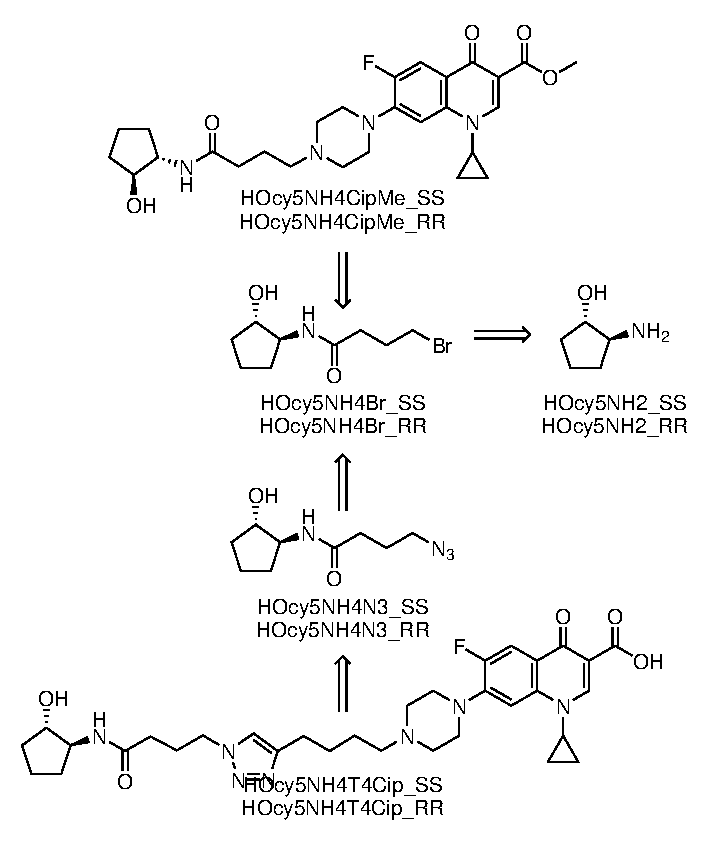
\includegraphics[scale=1]{HOcy5NH4_retro_A_wedges}
		\caption{Retrosynthesis of the cyclopentanol-CipMe conjugates 
		\compound{cmpd:HOcy5NH4CipMe_SS} (\textit{SS}) and 
		\compound{cmpd:HOcy5NH4CipMe_RR} (\textit{RR}),
		and the cyclopentanol-Cip triazole conjugates 
		\compound{cmpd:HOcy5NH4T4Cip_SS} (\textit{SS}) and  \compound{cmpd:HOcy5NH4T4Cip_RR} (\textit{RR}). 
		\textit{SS} enantiomers are shown, but both are implied. \label{sch:HOcy5NH4_retro_A}}
	\end{center}
\end{scheme}

Synthesis of Br-C$_4$-cyclopentanol-(\textit{SS}) \compound{cmpd:HOcy5NH4Br_SS} from (1\textit{S},2\textit{S})-2-aminocyclopentan-1-ol \compound{cmpd:HOcy5NH2_SS} and 4-bromobutyryl chloride \compound{cmpd:Cl4Br} was attempted using Schotten-Baumann conditions (see \ref{sch:HOcy5NH4Br_SS_synth}). However, a large number of impurities were observed by LCMS (see \ref{fig:HOcy5NH4Br_SS_impurities}), and so three new strategies were attempted: protection of the alcohol (see \ref{sec:TBDMS}), using 4-chlorobutyryl chloride \compound{cmpd:Cl4Cl} as the linker instead of 4-bromobutyryl chloride \compound{cmpd:Cl4Br} (see \ref{sec:Cl4Cl}), and  installing the linker on methyl ciprofloxacin \compound{cmpd:CipMe} and then attaching the head group by peptide coupling (see \ref{sec:CipMe_linker}).

%LMO-2-058

\begin{scheme}[H]
	\begin{center}
		\schemeref[HOcy5NH2]{cmpd:HOcy5NH2_SS}
		\schemeref[Cl4Br]{cmpd:Cl4Br}
		\schemeref[HOcy5NH4Br]{cmpd:HOcy5NH4Br_SS}
		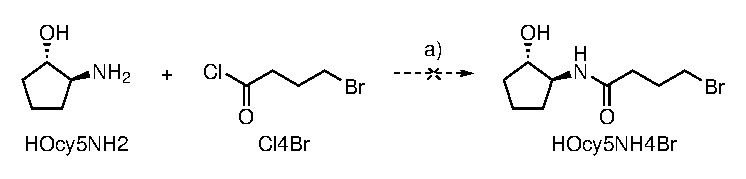
\includegraphics[scale=1]{HOcy5NH4Br_SS_synth}
		\caption{Attempted synthesis of Br-C$_4$-cyclopentanol-(\textit{SS}) \compound{cmpd:HOcy5NH4Br_SS}.
		a) \ce{NaHCO3}, \ce{CH2Cl2}, water, 0 $^{\circ}$C, 2 h. \label{sch:HOcy5NH4Br_SS_synth}}
	\end{center}
\end{scheme}

\begin{figure}[H]
	\begin{center}
		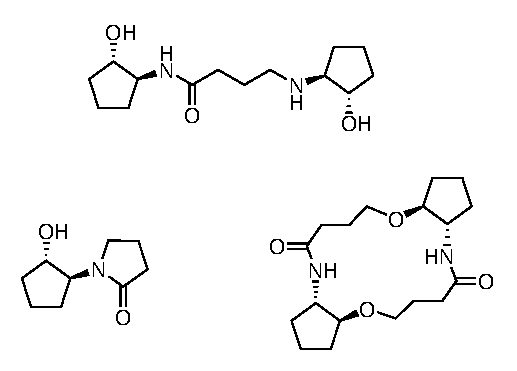
\includegraphics[scale=1]{HOcy5NH4Br_SS_impurities}
		\caption{Suspected impurities observed by LCMS during the synthesis of Br-C$_4$-cyclopentanol-(\textit{SS}) \compound{cmpd:HOcy5NH4Br_SS}.
		Regiochemistry is speculative.
		\label{fig:HOcy5NH4Br_SS_impurities}}
	\end{center}
\end{figure}

\subsubsection{TBDMS protection route \label{sec:TBDMS}}

The first attempt at an alternative strategy for the synthesis of the conjugates involved TBDMS protection of the alcohol (see \ref{sch:HOcy5NH4_retro_B}). It was envisaged that protection would eliminate enough of the side reactions with products shown in \ref{fig:HOcy5NH4Br_SS_impurities} that intermediates Br-C$_4$-cyclopentanol-(\textit{SS}) \compound{cmpd:HOcy5NH4Br_SS} and N$_3$-C$_4$-cyclopentanol-(\textit{SS}) \compound{cmpd:HOcy5NH4N3_SS} could be purified. The TBDMS group could be removed later in the synthesis using TBAF or acid.

\begin{scheme}[H]
	\begin{center}
		\schemeref[HOcy5NH2_RR]{cmpd:HOcy5NH2_RR}
		\schemeref[TBSOcy5NH2_RR]{cmpd:TBSOcy5NH2_RR}
		\schemeref[TBSOcy5NH4Br_RR]{cmpd:TBSOcy5NH4Br_RR}
		\schemeref[TBSOcy5NH4N3_RR]{cmpd:TBSOcy5NH4N3_RR}
		\schemeref[TBSOcy5NH4CipMe_RR]{cmpd:TBSOcy5NH4CipMe_RR}
		\schemeref[TBSOcy5NH4T4Cip_RR]{cmpd:TBSOcy5NH4T4Cip_RR}
		\schemeref[HOcy5NH4CipMe_RR]{cmpd:HOcy5NH4CipMe_RR}
		\schemeref[HOcy5NH4T4Cip_RR]{cmpd:HOcy5NH4T4Cip_RR}
		\schemeref[HOcy5NH2_SS]{cmpd:HOcy5NH2_SS}
		\schemeref[TBSOcy5NH2_SS]{cmpd:TBSOcy5NH2_SS}
		\schemeref[TBSOcy5NH4Br_SS]{cmpd:TBSOcy5NH4Br_SS}
		\schemeref[TBSOcy5NH4N3_SS]{cmpd:TBSOcy5NH4N3_SS}
		\schemeref[TBSOcy5NH4CipMe_SS]{cmpd:TBSOcy5NH4CipMe_SS}
		\schemeref[TBSOcy5NH4T4Cip_SS]{cmpd:TBSOcy5NH4T4Cip_SS}
		\schemeref[HOcy5NH4CipMe_SS]{cmpd:HOcy5NH4CipMe_SS}
		\schemeref[HOcy5NH4T4Cip_SS]{cmpd:HOcy5NH4T4Cip_SS}
		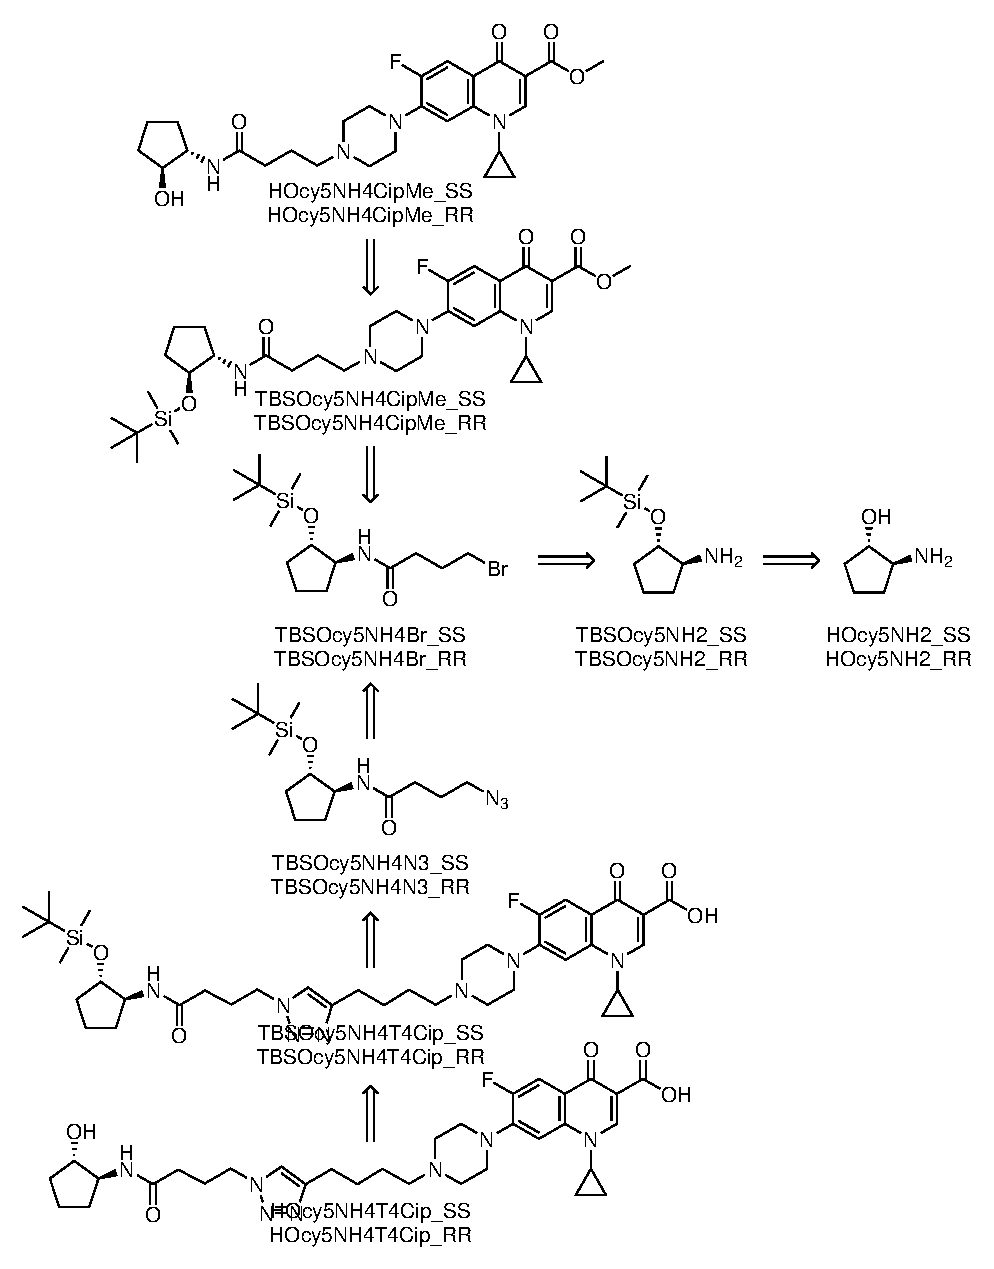
\includegraphics[scale=1]{HOcy5NH4_retro_B}
		\caption{Retrosynthesis of the cyclopentanol-CipMe conjugates 
		\compound{cmpd:HOcy5NH4CipMe_SS} (\textit{SS}) and  \compound{cmpd:HOcy5NH4CipMe_RR} (\textit{RR}), 
		and the cyclopentanol-Cip triazole conjugates 
		\compound{cmpd:HOcy5NH4T4Cip_SS} (\textit{SS}) and
		\compound{cmpd:HOcy5NH4T4Cip_RR} (\textit{RR}) 
		using a TBDMS protection strategy. \textit{SS} enantiomers are shown, but both are implied.\label{sch:HOcy5NH4_retro_B}}
	\end{center}
\end{scheme}

\subsubsubsection{Synthesis of TBDMS-protected (1\textit{S},2\textit{S})-2-aminocyclopentan-1-ol \compound{cmpd:HOcy5NH2_SS}}

The synthesis began with the optimisation of the protection of (1\textit{S},2\textit{S})-2-aminocyclopentan-1-ol \compound{cmpd:HOcy5NH2_SS} with a TBDMS group on the alcohol (see \ref{sch:TBSOcy5NH4Br_SS_synth}).
This reaction proved more problematic than expected, possibly due to the amine group interfering with the reaction at the alcohol and/or the high polarity of the starting material causing problems with solubility in the reaction mixture and extraction during the work-up. Conditions attempted are summarised in \ref{tbl:TBSOcy5NH4Br_SS_opt}. Protection attempts using TBDMSCl were generally unsuccessful, but eventually a method employed by Wu et. al\cite{Wu2012} using TBDMSOTf was found to produce the desired product in excellent yield. Water was used for the work-up rather than \ce{NH4Cl} (sat. aq.), as the acidic work-up protonated the product. The TEA was removed during column chromatography instead.


\begin{scheme}[H]
	\begin{center}
		\schemeref[HOcy5NH2]{cmpd:HOcy5NH2_SS}
		\schemeref[TBSOcy5NH2]{cmpd:TBSOcy5NH2_SS}
		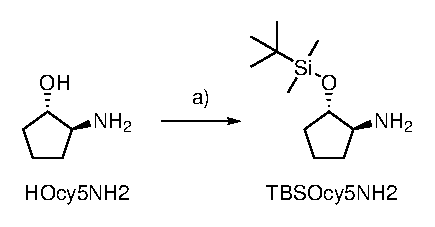
\includegraphics[scale=1]{TBSOcy5NH2_SS_synth}
		\caption{Synthesis of TBDMS protected (1\textit{S},2\textit{S})-2-aminocyclopentan-1-ol \compound{cmpd:TBSOcy5NH2_SS}. 
		a) See \ref{tbl:TBSOcy5NH4Br_SS_opt}.
		\label{sch:TBSOcy5NH2_SS_synth}}
	\end{center}
\end{scheme}

\renewcommand{\arraystretch}{1.2}
\begin{table}[H]
  \centering
\begin{tabular}{|p{6cm}|l|l|l|}
\hline 
Conditions & Temperature & Time & Result \\ 
\hline 
TBDMSCl, DMAP, TEA, \ce{CH2Cl2}\cite{Robak2007} & r.t. & 18 h & Trace of \compound{cmpd:TBSOcy5NH2_SS}, mostly \compound{cmpd:HOcy5NH2_SS} \\%LMO-2-060, LMO-2-067 
%\hline 
%TBDMSCl, DMAP, TEA, \ce{CH2Cl2} & r.t. & 1 d & Didn't go to completion, lost on prep TLC %LMO-2-063 \\ 
\hline 
TBDMSCl, imidazole, \ce{CH2Cl2}\cite{Yim2005} & 0 $^{\circ}$C & 1 h & \compound{cmpd:HOcy5NH2_SS} \\ %LMO-2-064, LMO-2-066
\hline 
TBDMSCl, DBU, acetonitrile \cite{Orsini1989} & 0 $^{\circ}$C & 1 d & \compound{cmpd:HOcy5NH2_SS} \\ %LMO-2-065
%\hline 
%TBDMSOTf, TEA, \ce{CH2Cl2} & 0 $^{\circ}$C & 4 h & \compound{cmpd:TBSOcy5NH2_SS} possibly seen but lost in workup \\ %LMO-2-062
%\hline 
%TBDMSOTf in 2 portions, TEA, \ce{CH2Cl2}, \ce{NH4Cl} workup & 0 $^{\circ}$C & 6 h & \compound{cmpd:TBSOcy5NH2_SS} salt \\ %LMO-2-068
\hline 
TBDMSOTf, TEA, \ce{CH2Cl2}\cite{Wu2012}, aq. workup then column & 0 $^{\circ}$C & 6 h & \compound{cmpd:TBSOcy5NH2_SS}, 98\% yield \\ %LMO-2-070, LMO-2-071
\hline 
\end{tabular} 
\caption{Conditions attempted for the synthesis of (1\textit{S},2\textit{S})-2-((\textit{tert}-butyldimethylsilyl)oxy)cyclopentan-1-amine \compound{cmpd:TBSOcy5NH2_SS} (see \ref{sch:TBSOcy5NH4Br_SS_synth}).\label{tbl:TBSOcy5NH4Br_SS_opt}} 
\end{table}

\subsubsubsection{Synthesis of Br-C$_4$-cyclopentanol-TBDMS-(\textit{SS}) \compound{cmpd:TBSOcy5NH4Br_SS}}

The TBDMS protected (1\textit{S},2\textit{S})-2-aminocyclopentan-1-ol \compound{cmpd:TBSOcy5NH2_SS} was reacted with 4-bromobutyryl chloride \compound{cmpd:Cl4Br} to form Br-C$_4$-cyclopentanol-TBDMS-(\textit{SS}) \compound{cmpd:TBSOcy5NH4Br_SS}. The reaction was observed to go to completion by TLC, but it became apparent that the product was reacting further during concentration and purification. Adding sodium azide to the mixture obtained after the failed purification attempts was observed to convert the remaining Br-C$_4$-cyclopentanol-TBDMS-(\textit{SS}) \compound{cmpd:TBSOcy5NH4Br_SS} to N$_3$-C$_4$-cyclopentanol-TBDMS-(\textit{SS}) \compound{cmpd:TBSOcy5NH4N3_SS}. 
A sequential one-pot reaction was therefore used, so that the reactive intermediate did not need to be isolated.
%073 078

\begin{scheme}[H]
	\begin{center}
		\schemeref[Cl4Br]{cmpd:Cl4Br}
		\schemeref[TBSOcy5NH2]{cmpd:TBSOcy5NH2_SS}
		\schemeref[TBSOcy5NH4Br]{cmpd:TBSOcy5NH4Br_SS}
		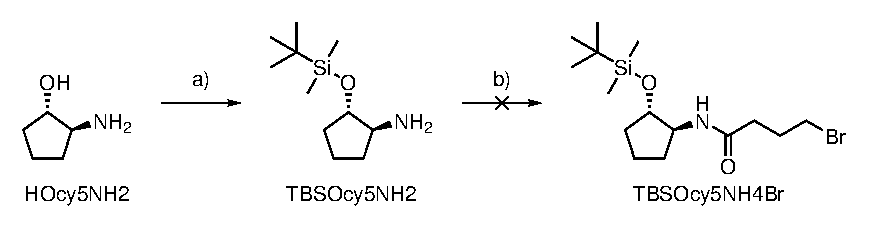
\includegraphics[scale=1]{TBSOcy5NH4Br_SS_synth}
		\caption{Attempted synthesis of Br-C$_4$-cyclopentanol-TBDMS-(\textit{SS}) \compound{cmpd:TBSOcy5NH4Br_SS}. 
		a) \ce{NaHCO3}, \ce{CH2Cl2}, water, 0 $^{\circ}$C, 2 h. %069,072,073
		\label{sch:TBSOcy5NH4Br_SS_synth}}
	\end{center}
\end{scheme}

\subsubsubsection{Synthesis of N$_3$-C$_4$-cyclopentanol-TBDMS-(\textit{SS}) \compound{cmpd:TBSOcy5NH4N3_SS} by one-pot reaction}

N$_3$-C$_4$-cyclopentanol-TBDMS-(\textit{SS}) \compound{cmpd:TBSOcy5NH4N3_SS} was finally synthesised by a two-step, one-pot reaction. Schotten-Baumann conditions were used to form the bromide. The water was then removed, and DMF and sodium azide were added. N$_3$-C$_4$-cyclopentanol-TBDMS-(\textit{SS}) \compound{cmpd:TBSOcy5NH4N3_SS} was produced in excellent yield.

\begin{scheme}[H]
	\begin{center}
		\schemeref[TBSOcy5NH2]{cmpd:TBSOcy5NH2_SS}
		\schemeref[Cl4Br]{cmpd:Cl4Br}
		\schemeref[TBSOcy5NH4Br]{cmpd:TBSOcy5NH4Br_SS}		\schemeref[TBSOcy5NH4N3]{cmpd:TBSOcy5NH4N3_SS}
		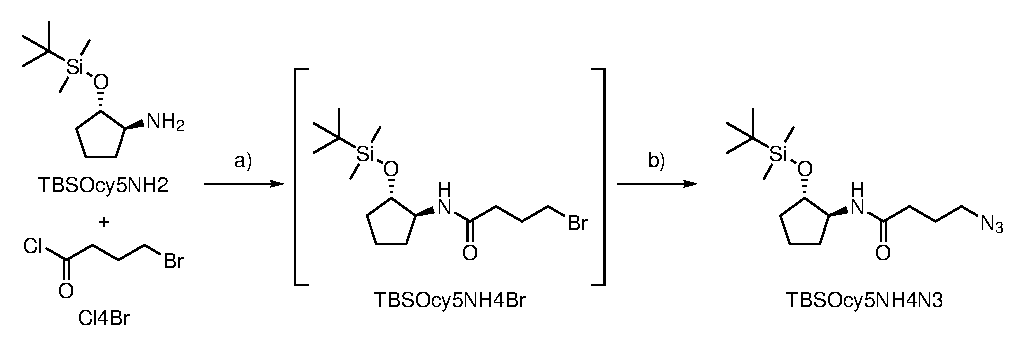
\includegraphics[scale=1]{TBSOcy5NH4N3_SS_synth_2step}
		\caption{
		Synthesis of N$_3$-C$_4$-cyclopentanol-TBDMS-(\textit{SS}) \compound{cmpd:TBSOcy5NH4N3_SS}.
		a) \ce{NaHCO3}, \ce{CH2Cl2}, water, 0 $^{\circ}$C, 3 h.
		b) \ce{NaN3}, DMF, \ce{CH2Cl2}, r.t., 3 h. 
		99\% over 2 steps. %LMO-2-078
		\label{sch:TBSOcy5NH4N3_SS_synth_2step}}
	\end{center}
\end{scheme}

\subsubsubsection{Synthesis of the (\textit{SS})-TBDMS-cyclopentanol-Cip triazole conjugate \compound{cmpd:TBSOcy5NH4T4Cip_SS}}

N$_3$-C$_4$-cyclopentanol-TBDMS-(\textit{SS}) \compound{cmpd:TBSOcy5NH4N3_SS} and the alkynyl ciprofloxacin derivative \compound{cmpd:Y4Cip} were subjected to standard click conditions (see \ref{sec:click_general}), and the (\textit{SS})-TBDMS-cyclopentanol-Cip triazole conjugate \compound{cmpd:TBSOcy5NH4T4Cip_SS} was synthesised in very good yield. However, removal of the TBDMS group proved difficult. Deprotection using 1.5 eq. TBAF in THF proceeded slowly, reaching completion in 5 d. Increasing the amount of TBAF to 8 eq. allowed the reaction to proceed overnight.
Purification of the final conjugate \compound{cmpd:HOcy5NH4T4Cip_SS} by column chromatography was not successful due to streaking and poor separation. Purification using DOWEX resin and \ce{CaCO3}\cite{Kaburagi2007} was attempted, but the product could not be recovered from the resin.
The purification method could probably be optimised, e.g. by varying the solvent used with the resin, but ultimately this route was abandoned due to the reduction in number of steps afforded by the two methods described below.

\begin{scheme}[H]
	\begin{center}
		\schemeref[TBSOcy5NH4N3]{cmpd:TBSOcy5NH4N3_SS}
		\schemeref[Y4Cip]{cmpd:Y4Cip}
		\schemeref[TBSOcy5NH4T4Cip]{cmpd:TBSOcy5NH4T4Cip_SS}
		\schemeref[HOcy5NH4T4Cip]{cmpd:HOcy5NH4T4Cip_SS}
		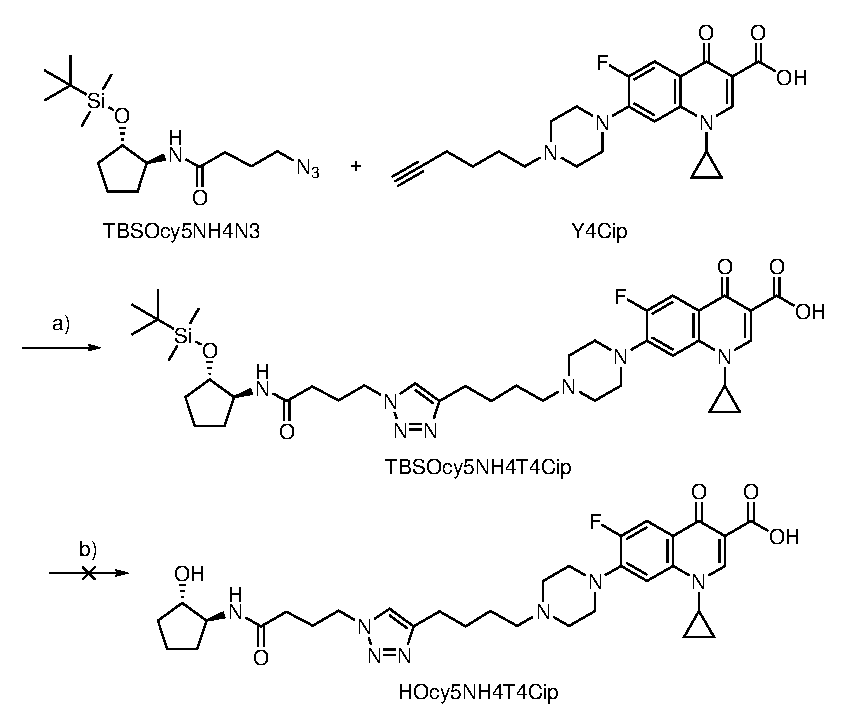
\includegraphics[scale=1]{TBSOcy5NH4T4Cip_SS_synth}
		\caption{Synthesis of the (\textit{SS})-TBDMS-cyclopentanol-Cip triazole conjugate \compound{cmpd:TBSOcy5NH4T4Cip_SS}.
		a) \ce{CuSO4}, sodium ascorbate, THPTA, water, \textit{t}-BuOH, r.t., 87\%. %, LMO-2-082
		b) TBAF, THF, r.t., 16 h. %LMO-2-084, 090, Lost on purification
		\label{sch:TBSOcy5NH4T4Cip_SS_synth}}
	\end{center}
\end{scheme}

\subsubsection{Synthesis of the cyclopentanol-Cip triazole conjugates \compound{cmpd:HOcy5NH4T4Cip_SS} and \compound{cmpd:HOcy5NH4T4Cip_RR} via chloride intermediates\label{sec:Cl4Cl}}

Given that the side product formation seen in the previous sections was most likely due to S$_N$2 attack on the bromide, we decided to use a chloride rather than a bromide intermediate (see \ref{sch:HOcy5NH4_retro_A} and \ref{sch:HOcy5NH4_retro_C} to compare). The bromide intermediate was initially chosen as it was used by Ganguly et. al\cite{Ganguly2011}, but it was anticipated that using a chloride would reduce the side reactions seen with the more reactive bromide.

\begin{scheme}[H]
	\begin{center}
		\schemeref[HOcy5NH2_SS]{cmpd:HOcy5NH2_SS}
		\schemeref[HOcy5NH4Cl_SS]{cmpd:HOcy5NH4Cl_SS}
		\schemeref[HOcy5NH4N3_SS]{cmpd:HOcy5NH4N3_SS}
		\schemeref[HOcy5NH4CipMe_SS]{cmpd:HOcy5NH4CipMe_SS}
		\schemeref[HOcy5NH4T4Cip_SS]{cmpd:HOcy5NH4T4Cip_SS}
		\schemeref[HOcy5NH2_RR]{cmpd:HOcy5NH2_RR}
		\schemeref[HOcy5NH4Cl_RR]{cmpd:HOcy5NH4Cl_RR}
		\schemeref[HOcy5NH4N3_RR]{cmpd:HOcy5NH4N3_RR}
		\schemeref[HOcy5NH4CipMe_RR]{cmpd:HOcy5NH4CipMe_RR}
		\schemeref[HOcy5NH4T4Cip_RR]{cmpd:HOcy5NH4T4Cip_RR}
		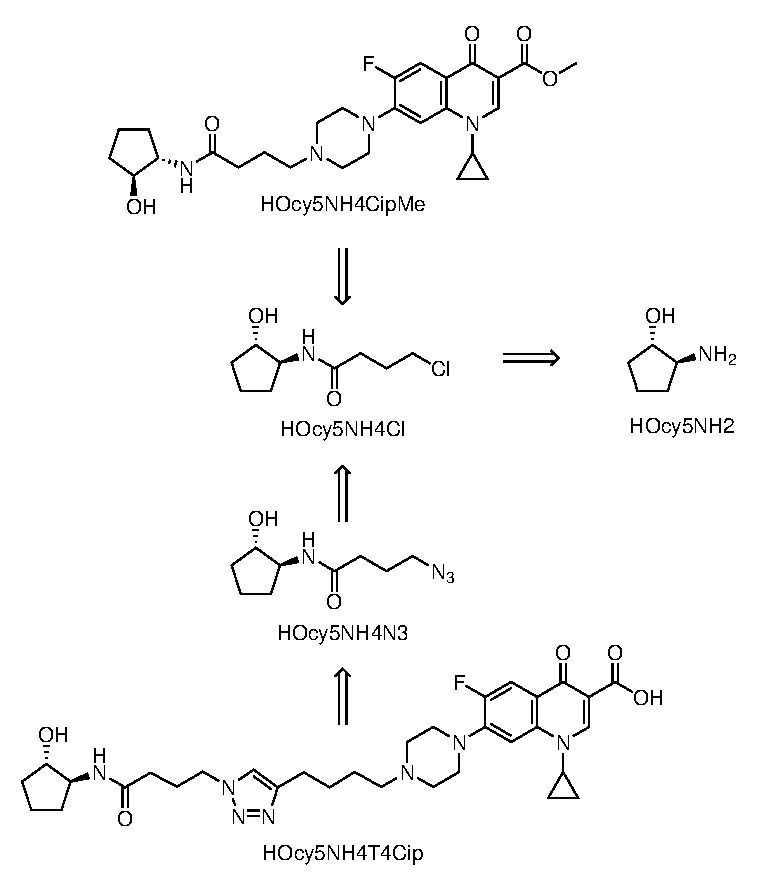
\includegraphics[scale=1]{HOcy5NH4_retro_C}
		\caption{Retrosynthesis of the cyclopentanol-CipMe conjugates 
		\compound{cmpd:HOcy5NH4CipMe_SS} (\textit{SS}) and
		\compound{cmpd:HOcy5NH4CipMe_RR} (\textit{RR}), 
		and the cyclopentanol-Cip triazole conjugates 
		\compound{cmpd:HOcy5NH4T4Cip_SS} (\textit{SS}) and
		\compound{cmpd:HOcy5NH4T4Cip_RR} (\textit{RR})  
		via Cl-C$_4$-cyclopentanol intermediates 
		\compound{cmpd:HOcy5NH4Cl_SS} (\textit{SS}) and 
		\compound{cmpd:HOcy5NH4Cl_RR} (\textit{RR}). 
		\textit{SS} enantiomers are shown, but both are implied.
		\label{sch:HOcy5NH4_retro_C}}
	\end{center}
\end{scheme}

Attempts at this route began with the synthesis of Cl-C$_4$-cyclopentanol-(\textit{RR}) \compound{cmpd:HOcy5NH4Cl_RR}. Standard Schotten-Baumann conditions failed to produce significant amounts of product. If prolonged reaction times were allowed, degradation of the acid chloride to the carboxylic acid was observed. The reason for this is unclear, but it is possible that bromide ions present in small amounts in previous reactions were helping to catalyse the reaction of the acid chloride. Archer \textit{et al.}\cite{Archer1953} propose that bromide ions can react with acid chlorides to form acid bromides, which are then more susceptible to nucleophilic attack.
As no bromide ions are present in this reaction, different conditions were sought in order to increase the rate.

As (1\textit{R},2\textit{R})-2-aminocyclopentan-1-ol \compound{cmpd:HOcy5NH2_RR} is fairly polar, it is likely that it was staying in the aqueous layer to some extent even when deprotonated, thus keeping the two reactants apart.
Therefore, the solvent system and base were changed to neat \ce{CH2Cl2} and TEA.
This produced Cl-C$_4$-cyclopentanol-(\textit{RR}) \compound{cmpd:HOcy5NH4Cl_RR} in good yield (64\%). Unlike the bromide \compound{cmpd:HOcy5NH4Br_SS}, the chloride \compound{cmpd:HOcy5NH4Cl_RR} was stable when concentrated.

Cl-C$_4$-cyclopentanol-(\textit{RR}) \compound{cmpd:HOcy5NH4Cl_RR} was converted to N$_3$-C$_4$-cyclopentanol-(\textit{RR}) \compound{cmpd:HOcy5NH4N3_RR} by reaction with sodium azide. The reaction was slower than with previous bromides (\textasciitilde16 h vs. \textasciitilde2 h), but much cleaner than with Br-C$_4$-cyclopentanol-(\textit{SS}) \compound{cmpd:HOcy5NH4Br_SS} (see \ref{sec:init_branch}).

The enantiomers Cl-C$_4$-cyclopentanol-(\textit{SS}) \compound{cmpd:HOcy5NH4Cl_SS} and N$_3$-C$_4$-cyclopentanol-(\textit{SS}) \compound{cmpd:HOcy5NH4N3_SS} were synthesised in lower yields, in part because of the smaller amounts being used.

\begin{scheme}[H]
	\begin{center}
		\schemeref[HOcy5NH2_SS]{cmpd:HOcy5NH2_SS}
		\schemeref[Cl4Cl]{cmpd:Cl4Cl}
		\schemeref[HOcy5NH4Cl_SS]{cmpd:HOcy5NH4Cl_SS}
		\schemeref[HOcy5NH4N3_SS]{cmpd:HOcy5NH4N3_SS}
		\schemeref[HOcy5NH2_RR]{cmpd:HOcy5NH2_RR}
		\schemeref[HOcy5NH4Cl_RR]{cmpd:HOcy5NH4Cl_RR}
		\schemeref[HOcy5NH4N3_RR]{cmpd:HOcy5NH4N3_RR}
		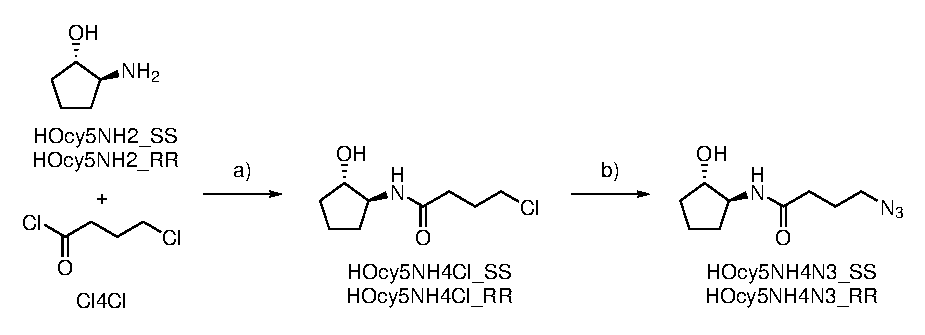
\includegraphics[scale=1]{HOcy5NH4N3_synth}
		\caption{Synthesis of N$_3$-C$_4$-cyclopentanol-(\textit{SS}) \compound{cmpd:HOcy5NH4N3_SS} and N$_3$-C$_4$-cyclopentanol-(\textit{RR}) \compound{cmpd:HOcy5NH4N3_RR}. 
		\textit{SS} enantiomers are shown, but both were synthesised.
		a) TEA, \ce{CH2Cl2}, 0 $^{\circ}$C, 2 h,
		\compound{cmpd:HOcy5NH4Cl_SS} (\textit{SS}): 24\%, 
		\compound{cmpd:HOcy5NH4Cl_RR} (\textit{RR}): 64\%.
		b) \ce{NaN3}, acetonitrile, 50 $^\circ$C, 16 h, 
		\compound{cmpd:HOcy5NH4N3_SS} (\textit{SS}): 45\%, 
		\compound{cmpd:HOcy5NH4N3_RR} (\textit{RR}): 88\%.
		\label{sch:HOcy5NH4N3_synth}}
	\end{center}
\end{scheme}

The cyclopentanol-Cip triazole conjugates \compound{cmpd:HOcy5NH4T4Cip_SS} (\textit{SS}) and \compound{cmpd:HOcy5NH4T4Cip_RR} (\textit{RR}) were successfully synthesised using standard click conditions (see \ref{sec:click_general}). 
Despite low yields (presumably due to problems with purification, including losses on the preparative HPLC column and high polarity leading to losses during extraction from aqueous solvents) enough of the compounds were obtained for biological testing so the purification was not optimised further.

\begin{scheme}[H]
	\begin{center}
		\schemeref[HOcy5NH4N3_SS]{cmpd:HOcy5NH4N3_SS}
		\schemeref[Y4Cip]{cmpd:Y4Cip}
		\schemeref[HOcy5NH4T4Cip_SS]{cmpd:HOcy5NH4T4Cip_SS}
		\schemeref[HOcy5NH4N3_RR]{cmpd:HOcy5NH4N3_RR}
		\schemeref[HOcy5NH4T4Cip_RR]{cmpd:HOcy5NH4T4Cip_RR}
		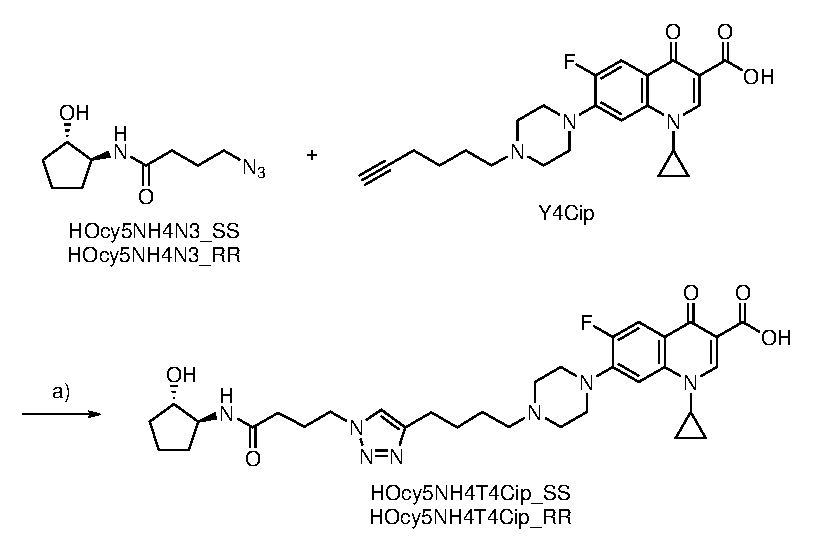
\includegraphics[scale=1]{HOcy5NH4T4Cip_synth}
		\caption{Synthesis of the cyclopentanol-Cip triazole conjugates \compound{cmpd:HOcy5NH4T4Cip_SS} (\textit{SS}) and 
		\compound{cmpd:HOcy5NH4T4Cip_RR} (\textit{RR}). 
		\textit{SS} enantiomers are shown, but both were synthesised.
		a) \ce{CuSO4}, THPTA, sodium ascorbate, water, \textit{t}-BuOH, r.t., 16 h, 
		\compound{cmpd:HOcy5NH4T4Cip_SS} (\textit{SS}): 22\%,
		\compound{cmpd:HOcy5NH4T4Cip_RR} (\textit{RR}): 27\%. 
		\label{sch:HOcy5NH4T4Cip_synth}}
	\end{center}
\end{scheme}

The S$_N$2 reaction of Cl-C$_4$-cyclopentanol-(\textit{RR}) \compound{cmpd:HOcy5NH4Cl_RR} and methyl ciprofloxacin \compound{cmpd:CipMe} was attempted (see \ref{sch:HOcy5NH4CipMe_SN2}) using the microwave conditions described previously (see \ref{sec:2MeO}), to see if the chloride produced better results compared with the bromide. However, as was seen with the other microwave reactions, a substantial amount of the disubstituted product \compound{cmpd:(HOcy5NH4)2CipMe+_RR} was seen by LCMS (in an approx 1:1 ratio with the desired product \compound{cmpd:HOcy5NH4CipMe}). 

\begin{scheme}[H]
	\begin{center}
		\schemeref[HOcy5NH4Cl_RR]{cmpd:HOcy5NH4Cl_RR}
		\schemeref[CipMe]{cmpd:CipMe}
		\schemeref[HOcy5NH4CipMe_RR]{cmpd:HOcy5NH4CipMe_RR}
		\schemeref[(HOcy5NH4)2CipMe+_RR]{cmpd:(HOcy5NH4)2CipMe+_RR}
		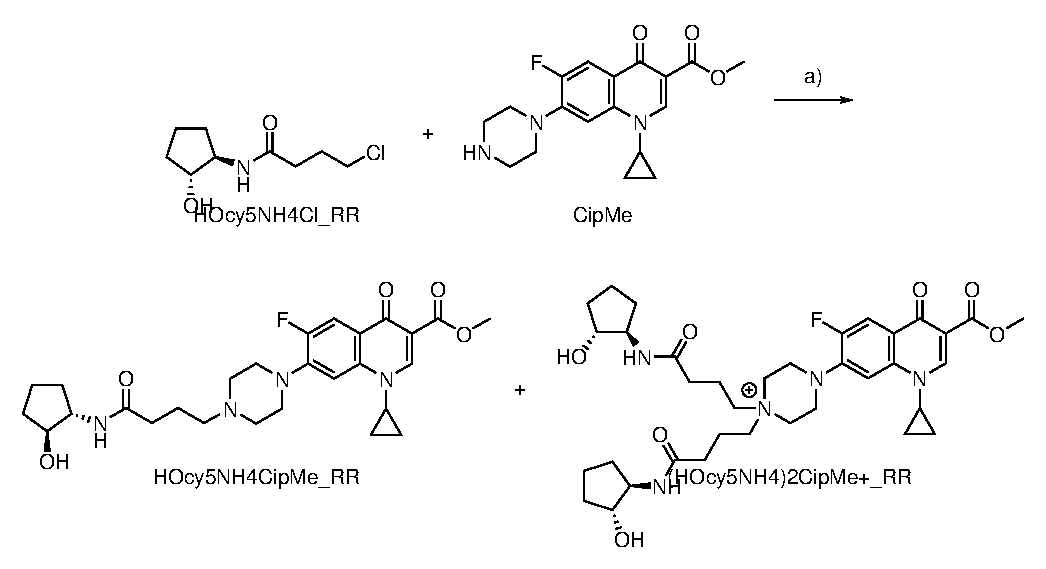
\includegraphics[scale=1]{HOcy5NH4CipMe_SN2}
		\caption{Attempted synthesis of the cyclopentanol-CipMe-(\textit{RR}) conjugate \compound{cmpd:HOcy5NH4CipMe_RR}.
		a) \ce{NaI}, DIPEA, acetonitrile, microwave reactor, 100 $^{\circ}$C.
		\label{sch:HOcy5NH4CipMe_SN2}}
	\end{center}
\end{scheme}

\subsubsection{Synthesis of the cyclopentanol-CipMe conjugates  \compound{cmpd:HOcy5NH4CipMe_SS} and \compound{cmpd:HOcy5NH4CipMe_RR} by peptide coupling\label{sec:CipMe_linker}}

Given the side-reactions and low yields associated with the literature synthesis of the S$_N$2 conjugates proposed by Ganguly et. al\cite{Ganguly2011}, an alternative synthesis was investigated, involving building up the linker on the ciprofloxacin side before coupling with the head group (see \ref{sch:HOcy5NH4_retro_D}).

%This was tested with _RR

\begin{scheme}[H]
	\begin{center}
		\schemeref[HOcy5NH2_SS]{cmpd:HOcy5NH2_SS}
		\schemeref[HOcy5NH2_RR]{cmpd:HOcy5NH2_RR}
		\schemeref[HOO4CipMe]{cmpd:HOO4CipMeTFA}
		\schemeref[tBuOO4CipMe]{cmpd:tBuOO4CipMe}
		\schemeref[tBuOO4Br]{cmpd:tBuOO4Br}
		\schemeref[CipMe]{cmpd:CipMe}
		\schemeref[HOcy5NH4CipMe_SS]{cmpd:HOcy5NH4CipMe_SS}
		\schemeref[HOcy5NH4CipMe_RR]{cmpd:HOcy5NH4CipMe_RR}
		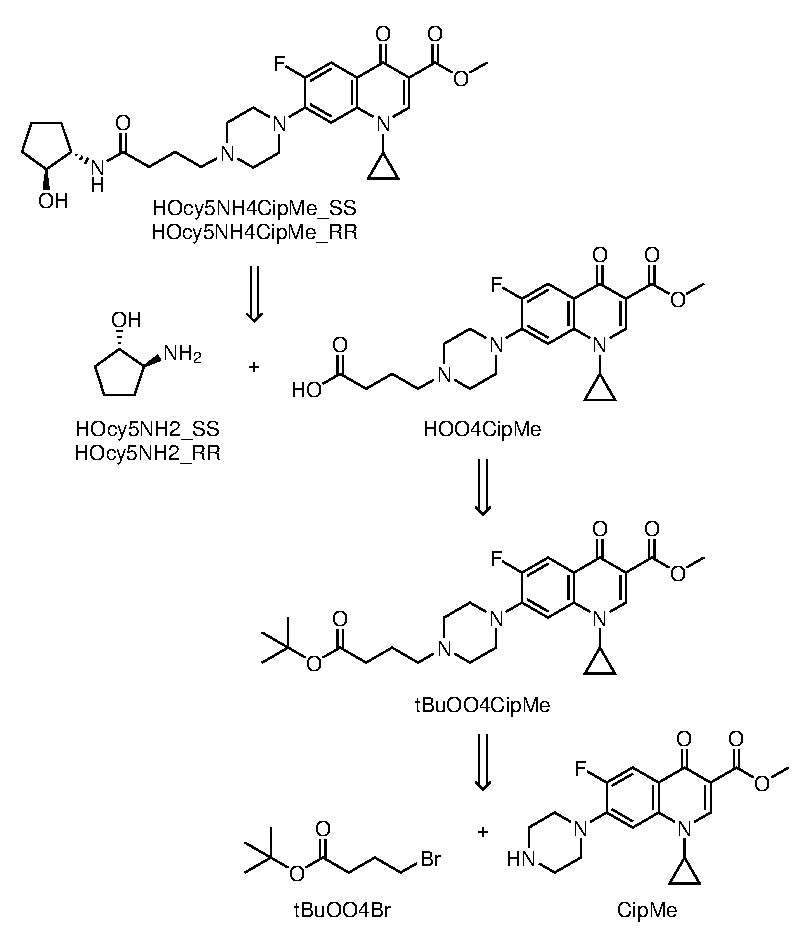
\includegraphics[scale=1]{HOcy5NH4_retro_D}
		\caption{Retrosynthesis of the cyclopentanol-CipMe conjugates  \compound{cmpd:HOcy5NH4CipMe_SS} (\textit{SS}) and \compound{cmpd:HOcy5NH4CipMe_RR} (\textit{RR}). \textit{SS} enantiomers are shown, but both are implied.\label{sch:HOcy5NH4_retro_D}}
	\end{center}
\end{scheme}

%a
The first step of the synthesis was an S$_N$2 reaction between Boc-protected 4-bromobutyric acid \compound{cmpd:tBuOO4Br} methyl ciprofloxacin \compound{cmpd:CipMe} (see \ref{sch:HOcy5NH4CipMe_RR_synth}). Intermediate \compound{cmpd:tBuOO4CipMe} was obtained in acceptable yield after column chromatography (50\%).
%b
Intermediate \compound{cmpd:tBuOO4CipMe} was deprotected in excellent yield using TFA in \ce{CH2Cl2} to give carboxylic acid \compound{cmpd:HOO4CipMeTFA}. Scale-up of this reaction allowed the easy synthesis of 600 mg of this useful intermediate, which can be coupled with various amine head-groups to create a library.
%c
Carboxylic acid \compound{cmpd:HOO4CipMeTFA} was first coupled with (1\textit{R},2\textit{R})-2-aminocyclopentan-1-ol \compound{cmpd:HOcy5NH2_RR} using standard peptide coupling conditions to give cyclopentanol-CipMe conjugate \compound{cmpd:HOcy5NH4CipMe_RR}. Purification by column chromatography was attempted twice with poor results, before moving on to using preparative HPLC, which gave \compound{cmpd:HOcy5NH4CipMe_RR} cleanly in 39\% yield.
Coupling was also performed with (1\textit{S},2\textit{S})-2-aminocyclopentan-1-ol \compound{cmpd:HOcy5NH2_SS} to give the enantiomer \compound{cmpd:HOcy5NH4CipMe_SS} in 55\% yield.



\begin{scheme}[H]
	\begin{center}
		\schemeref[CipMe]{cmpd:CipMe}
		\schemeref[tBuOO4Br]{cmpd:tBuOO4Br}
		\schemeref[tBuOO4CipMe]{cmpd:tBuOO4CipMe}
		\schemeref[HOO4CipMe]{cmpd:HOO4CipMeTFA}
		\schemeref[HOcy5NH2_SS]{cmpd:HOcy5NH2_SS}
		\schemeref[HOcy5NH2_RR]{cmpd:HOcy5NH2_RR}
		\schemeref[HOcy5NH4CipMe_SS]{cmpd:HOcy5NH4CipMe_SS}
		\schemeref[HOcy5NH4CipMe_RR]{cmpd:HOcy5NH4CipMe_RR}
		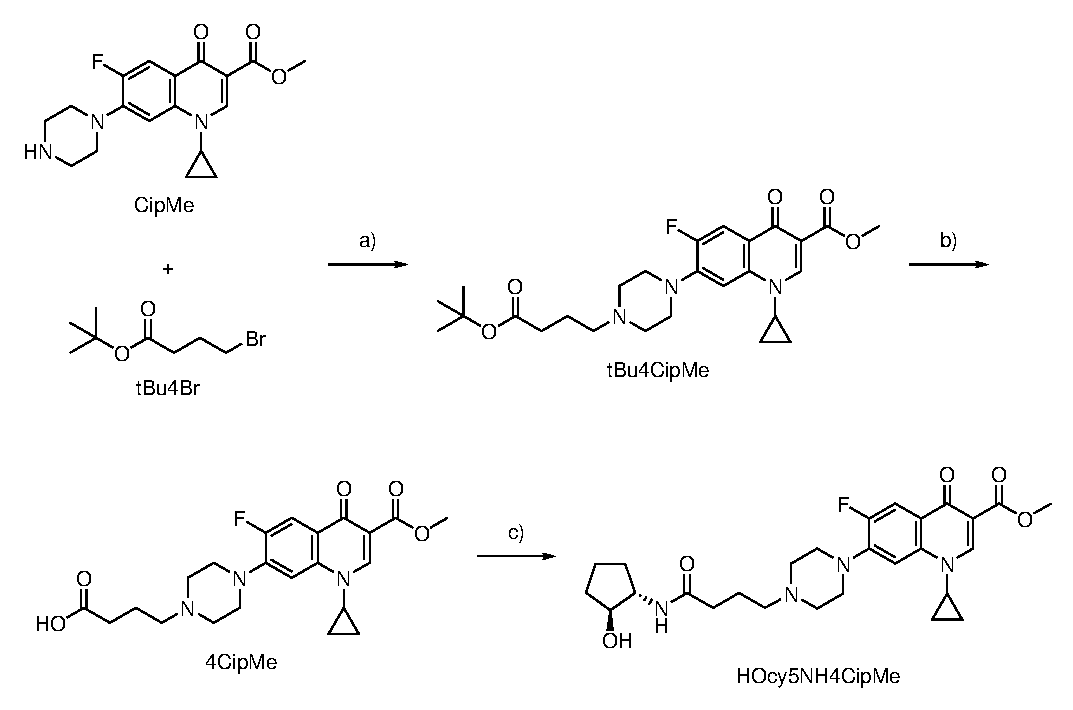
\includegraphics[scale=1]{HOcy5NH4CipMe_RR_synth}
		\caption{Synthesis of the cyclopentanol-CipMe conjugates  \compound{cmpd:HOcy5NH4CipMe_SS} (\textit{SS}) and \compound{cmpd:HOcy5NH4CipMe_RR} (\textit{RR}) by peptide coupling. 
		\textit{SS} enantiomers are shown, but both were synthesised.
			a) NaI, TEA, acetonitrile, 100 $^{\circ}$C, 16 h, 50\%. %, LMO-2-081
			b) TFA,  \ce{CH2Cl2}, r.t., 18 h, 96\%. %, LMO-2-083. 
			c) EDC, HOBt, DIPEA, DMF, r.t., 16 h, 
			\compound{cmpd:HOcy5NH4CipMe_SS} (\textit{SS}): 55\%,  %LMO-3-019
			\compound{cmpd:HOcy5NH4CipMe_RR} (\textit{RR}): 39\%. %LMO-2-093
			\label{sch:HOcy5NH4CipMe_RR_synth}}
	\end{center}
\end{scheme}





With (unfortunately not branching) routes to the S$_N$2 and click conjugates established (see \ref{sec:CipMe_linker} and \ref{sec:Cl4Cl} respectively), attention was turned to the cyclohexanol derivatives.